Most music notation programs have a visual approach, in which the user drags and drops notes and
symbols using the mouse and the resulting sheet is displayed on the screen.

An alternative approach is writing music using a text-based notation. This is a non-visual mode that
represents notes and other symbols using text characters, making it economic and sometimes intuitive
to use and also making possible faster transcriptions. A specialized program then translates the
notation into printable sheet music in some electronic format (e.g. PDF) and/or into a \midi{} file.

The three most known text-based notations are \abc{}~\cite{abcnotation:Online},
LilyPond~\cite{lilypond:Online} and MusicXML~\cite{musicxml:Online}.

\subsection{ABC}

\abc{} was introduced by Chris Walshaw in 1991 as a means to share traditional folk music, such as
Irish jigs. It was later expanded to provide multiple voices (polyphony), page layout details, and
\midi{} commands. \abc{} is a musical notation standard and not a software package meaning that it
depends on external tools to produce a printable sheet or a \midi{} file.

An \abc{} tune has a header with fields for title (T), composer (C), key signature (K), time
signature or meter (M) and default note duration or length (L). The music is notated using the
letters \emph{A} (\textit{lá}) to \emph{G} (\textit{sol}) to represent the notes.

The notation has a simple and clean syntax, and is powerful enough to produce professional and
complete music scores. The most important advantages are presented:

\begin{itemize}
  \item powerful enough to describe most music scores available in paper;
  \item actively maintained and developed;
  \item the source files are plain text files;
  \item easy searching and indexing of tune books and easy creation of music archives;
  \item it can be easily converted to other known formats;
  \item there are already tools for transforming and publishing \abc{}, such as,
    \abcmtops{}~\cite{abcm2ps:Online} (produces sheet music scores in PostScript or SVG) and
    \abctomidi{}~\cite{abc2midi:Online} (produces a \midi{} file);
  \item compact and clear notation;
  \item human readable;
  \item thousands of tunes available on the Internet;
  \item open source.
\end{itemize}

\abc{} was adopted in this dissertation in order to cope with real world problems that occurred in
the project WikiScore~\cite{almeida2012wiki}. Listing \ref{lst:abc_example} illustrates an example
of \abc{} notation and figure \ref{fig:abc_example} its corresponding score (the first
section's \emph{Soprano} part of the \emph{Christmas Villancico}\footnote{A Villancico is a musical
and poetic form written in Spanish and Portuguese, traditional from Spain, Latin America and
Portugal. These pieces were popular between century XV and XVIII.} \textit{Verbum caro factum est}).

\lstinputlisting[caption={\abc{} example},label={lst:abc_example},captionpos=t,abovecaptionskip=-\medskipamount,float]{misc/verbum_s1_p1.tex}

\vspace{-0.25cm}
\begin{figure}[htb]
  \centering
  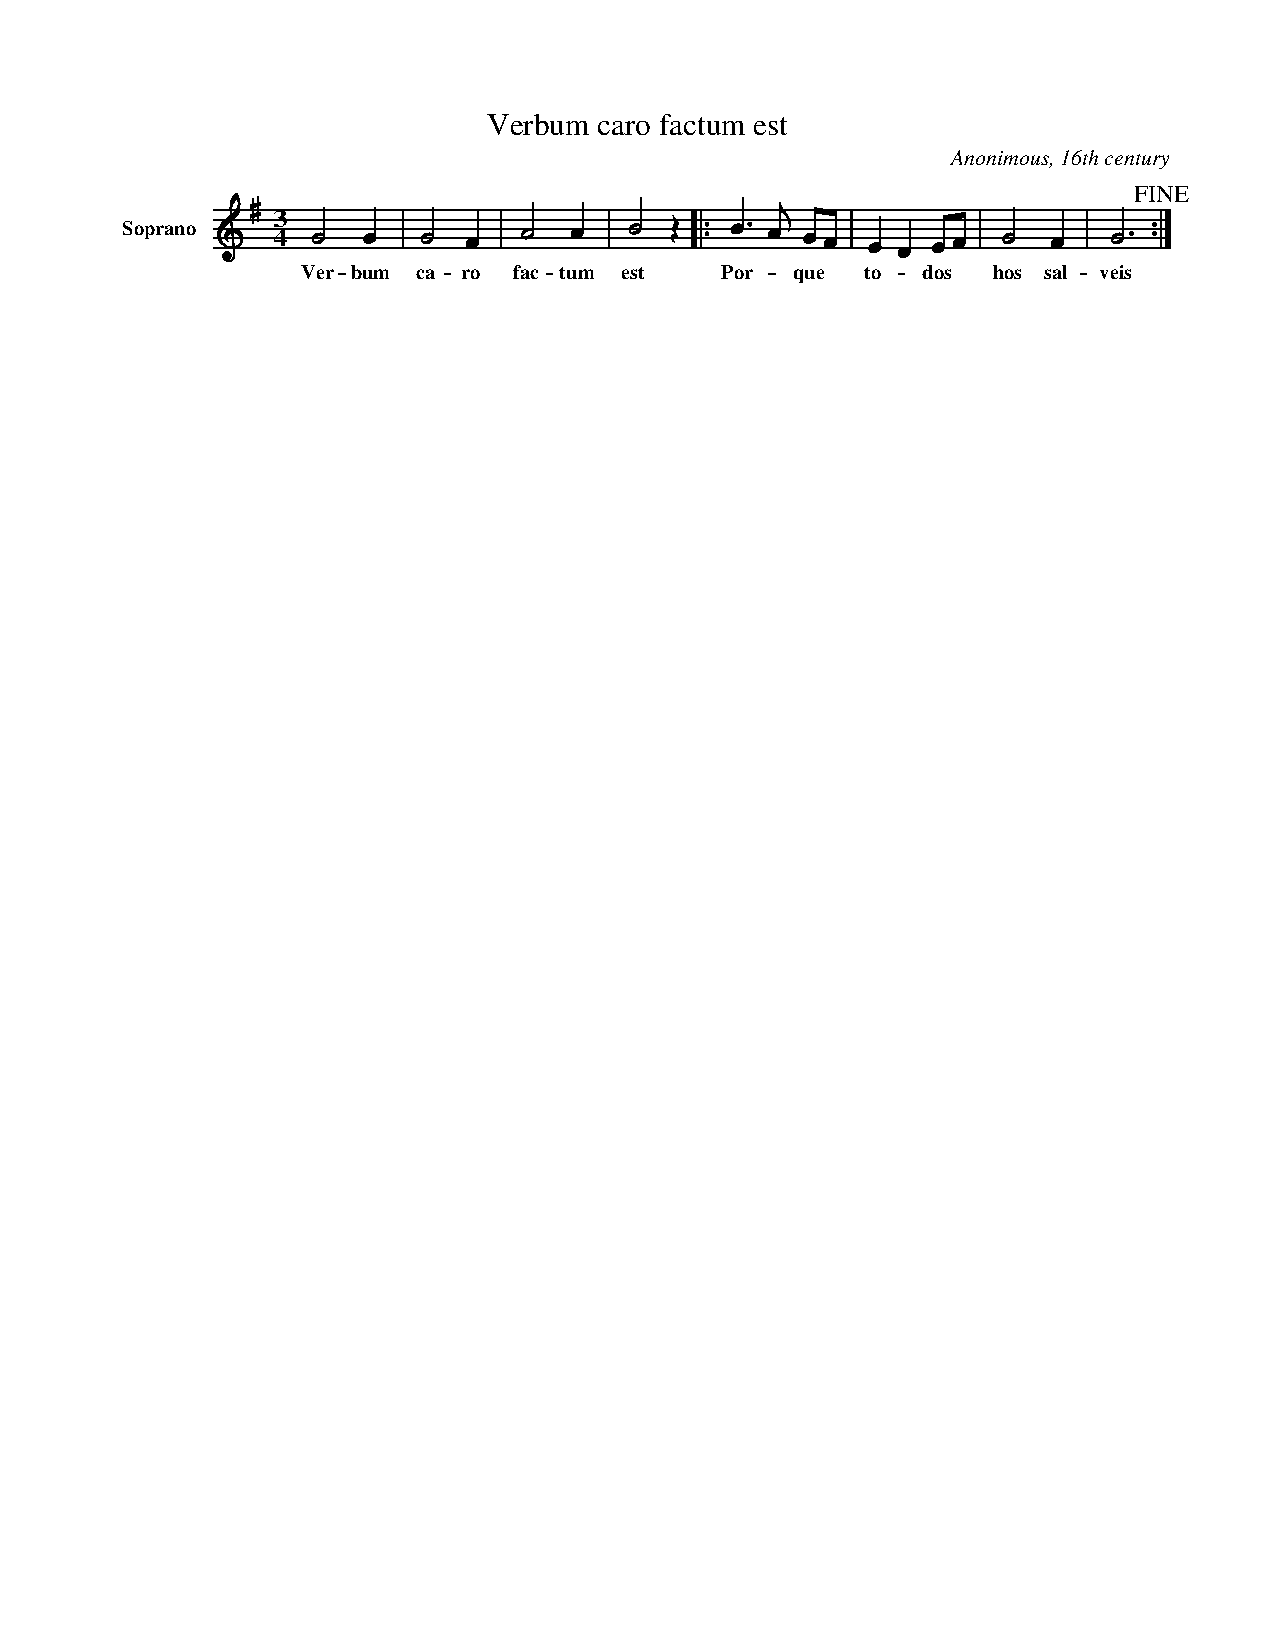
\includegraphics[width=0.8\textwidth, clip=true, trim = 0mm 230mm 0mm 17mm]{img/101.pdf}
  \caption{\abc{} example's generated score}
  \label{fig:abc_example}
\end{figure}

There are many \abcpt{}s and, among them, the most popular are the typesetter
\abcmtops{}~\cite{abcm2ps:Online} and the \midi{} creator \abctomidi{}~\cite{abc2midi:Online}. The
first translates music written in \abc{} into customary sheet music scores in PostScript or SVG
format. The latter converts an \abc{} file into a \midi{} file.

\subsection{LilyPond}

GNU LilyPond\cite{lilypond:Online} is a computer program and file format for music engraving. It
formats music beautifully and automatically, and has a friendly syntax for its input files. It is
Free Software, this is, open source. One of LilyPond's major goals is to produce scores that are
engraved with traditional layout rules, reflecting the era when scores were engraved by hand.

Although there are some small similarities to \abc{}, there are significant differences, starting
with their intent. \abc{}'s original purpose was to create a simple means of sharing folk tunes that
could be read as text and sent as email. Besides, it is a music notation standard, not a software
package. LilyPond is a software with the intent of creating printed musical scores that match the
best hand engraved musical scores of the past.

The similarity between \abc{} and LilyPond is in the means of specifying notes in a musical score,
this is, through the letters \emph{A} to \emph{G}.

LilyPond has a much more ambitious goal than \abc{}, therefore the markup language for its source
file can quickly become complex if the goal is to combine, for instance, melody, tab, chords, chord
diagrams and lyrics.

Listing \ref{lst:verbum_s1_p1_ly} illustrates the same example used for \abc{} using LilyPond
notation and figure \ref{fig:verbum_s1_p1_score_ly} its corresponding score.\\

\lstinputlisting[caption={LilyPond Example},label={lst:verbum_s1_p1_ly},captionpos=t,abovecaptionskip=-\medskipamount]{misc/verbum_s1_p1_ly.tex}

\vspace{-0.25cm}
\begin{figure}[htb]
  \centering
  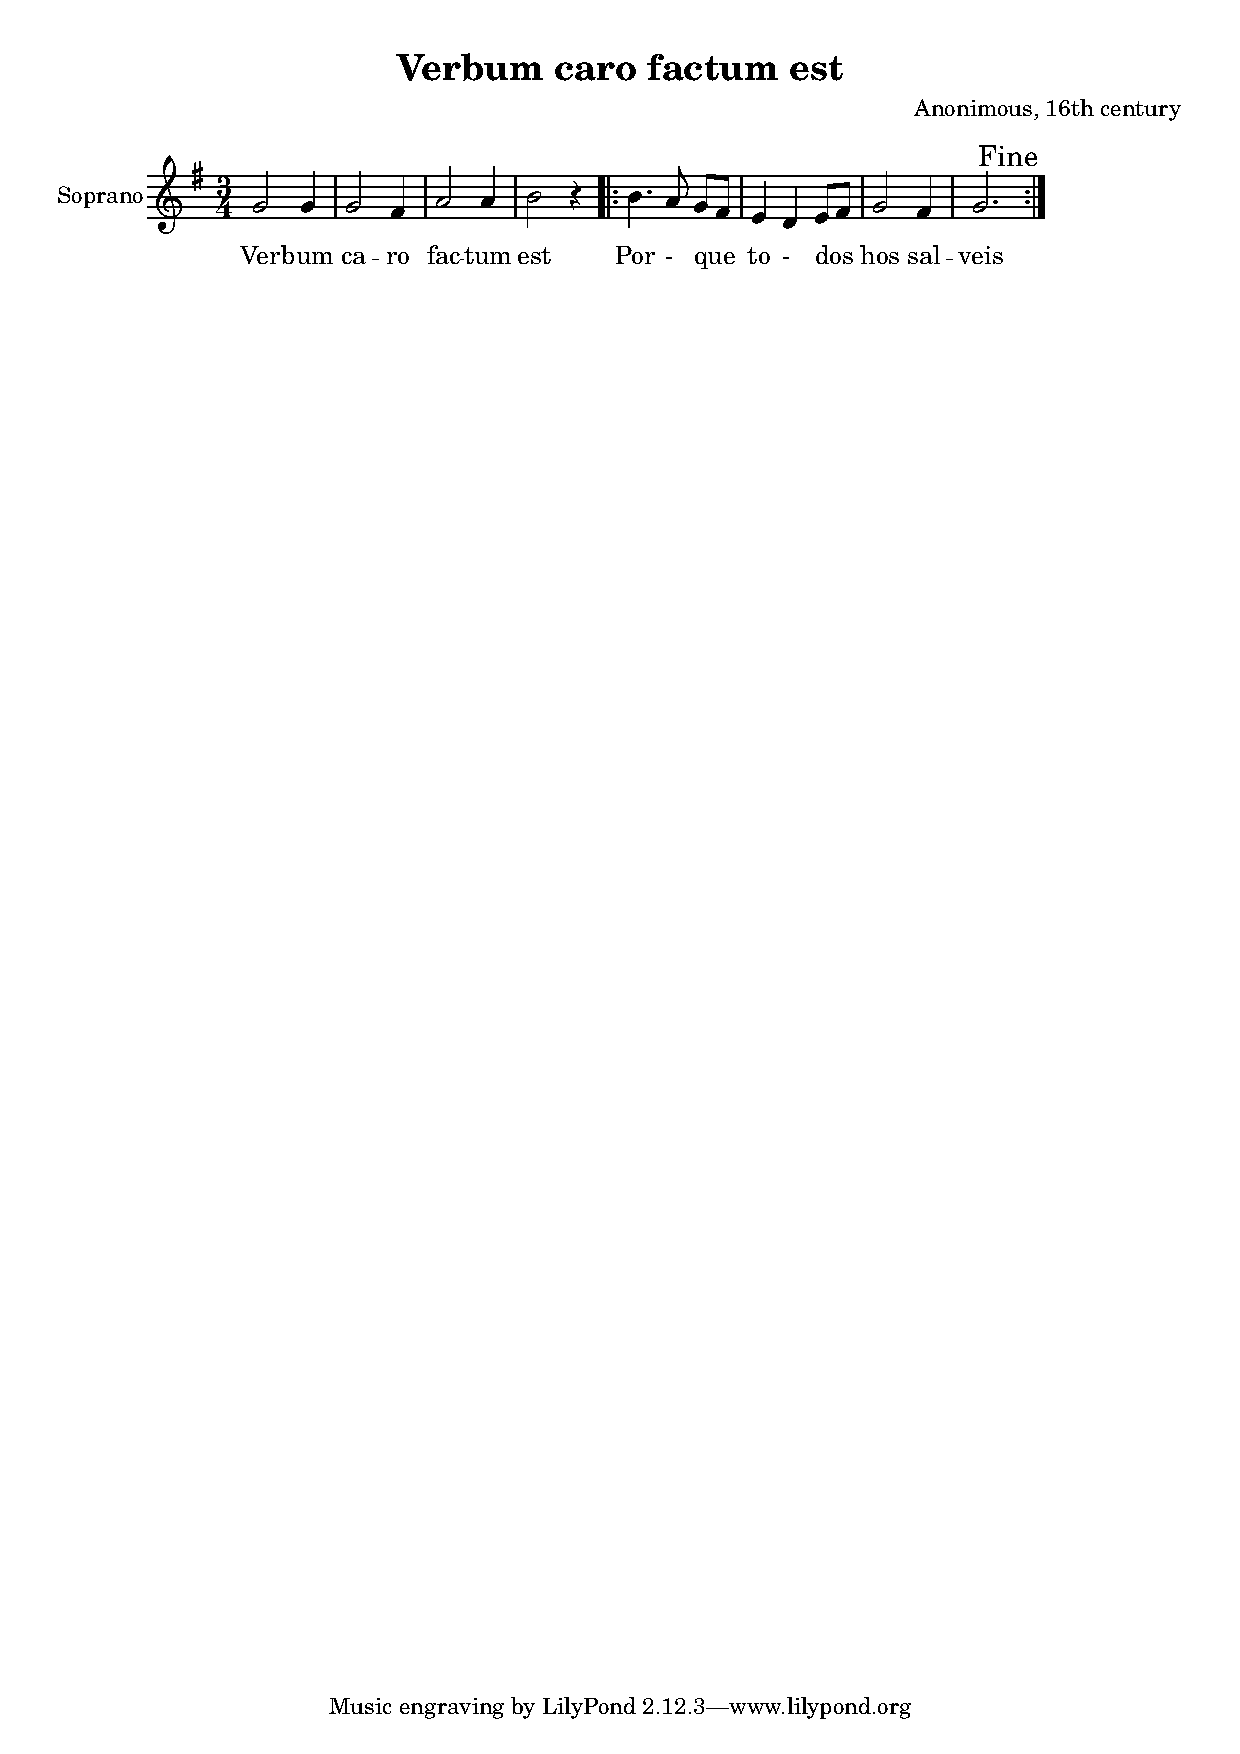
\includegraphics[width=0.8\textwidth, clip=true, trim = 9mm 250mm 9mm 6mm]{img/verbum_s1_p1_ly.pdf}
  \caption{LilyPond example's generated score}
  \label{fig:verbum_s1_p1_score_ly}
\end{figure}

\subsection{MusicXML}

MusicXML\cite{musicxml:Online} is an XML-based file format for representing Western musical notation
designed for notation, analysis, retrieval, and performance applications. The format is proprietary,
developed by Recordare LLC, but fully and openly documented, and can be freely used under a Public
License.

MusicXML was designed from the ground up for sharing sheet music files between different
applications, and for archiving sheet music files for use in the future. Its files are readable and
usable by a wide range of music notation applications, now and in the future. MusicXML complements
the native file formats used by Finale~\cite{Finale:Online} and other
programs~\cite{Sibelius:Online}, which are designed for rapid, interactive use.
